\chapter{引言}
\section{问题介绍}

在当今数字图像处理和计算机视觉领域,图像去噪一直是一个至关重要的问题。在实际应用中,由于各种因素,例如传感器噪声、压缩、低光条件等,图像中常常存在噪声,这会影响到图像的质量和后续处理任务的准确性。以及受限于测量仪器的局限性,测量采样得到的图像相比于原始图像也会存在相对误差,如何从现实中实际获取带噪图像中还原得到原先清晰度更高的原始图像具有重大的应用价值和前景。     

尽管目前已经有诸如扩散模型为代表的图像去噪基础模型,但是其采样时间较长限制了其在工业生产中的大规模应用。 如何在时间以及算力资源限制下更高效地对获取到的图像进行去噪还原得到原始图像,如何获取超分辨率的图像?这些都是在实际工业领域应用较为重要的实际问题。 
因此,开发高效准确的图像去噪算法对于提升图像质量以及下游任务的性能具有重要意义。
\subsection*{图像去噪的挑战}
传统的图像去噪方法通常基于滤波器和统计学方法,它们可以在某些场景下取得不错的效果。然而,在面对复杂的噪声分布或者噪声与信号之间相互重叠的情况下,传统方法的性能往往受到限制。特别是对于低信噪比(SNR)的图像,传统方法可能会产生过度平滑或者细节损失的问题。      

若利用传统统计学习方法来进行图像处理,则通常将二维图像当作一维向量进行处理。图像作为一类特殊的数据类型其分布通常可以被看作在高维向量空间中的一个低维流形的嵌入,即在图像中通常有较多常见特征反复出现,使得其有相比于一般向量空间中数据分布的特殊性质,若对其向量化则会失去一部分图像数据分布独有的特征。在传统图像去噪研究中,例如\cite{DZGS202401008}采用结合高斯滤波和在波域进行迭代的算法对图像进行修复还原,但是该类型图像修复算法对初识输入的噪声较为敏感,无法对较为复杂的图像去噪下游任务进行还原(例如对图像一整块区域进行挖除的图像修复任务)。
\subsection*{引入深度学习}
近年来,随着深度学习技术的发展,基于深度学习的图像去噪方法逐渐受到关注。随着现代深度学习方法的发展,其中,Variational Autoencoder(VAE)和Diffusion Model (DM)等深度生成模型因其能够学习到图像的复杂概率分布而备受瞩目。这些模型不仅能够准确地去除噪声,还可以保留图像的细节和结构,从而在实际应用中取得更好的效果。以及随着最新提出的大语言模型(LLM), 可以借助现有的大模型对图像进行切割,利用语义分割对对不同部分进行分开处理训练,从而获得更高的图像质量,其中在\cite{DM_review}中就详细分别介绍了在VAE模型以及在大语言模型下的图像修复算法。 
\section{选题背景及意义}

\subsection*{选题背景}
随着数字图像在日常生活和工业应用中的普及,图像质量的要求越来越高。然而,在现实世界中,图像往往会受到各种形式的干扰和噪声,例如传感器噪声、压缩引起的伪像、低光条件下的图像模糊等。这些噪声不仅降低了图像的质量,还可能影响后续的图像分析和处理任务的准确性和可靠性。    


传统的图像去噪方法通常基于数学模型和信号处理技术,例如中值滤波、高斯滤波,卷积张量等。然而,这些方法往往只能处理特定类型的噪声,对于复杂的噪声分布或者噪声与信号之间的相互干扰,传统方法的效果可能不尽如人意,具有较大的局限性。
\subsection*{选题意义}
提升图像质量的关键在于实施高效的图像去噪算法,这些算法能够显著改善图像的清晰度和真实感,从而极大增强用户的观感体验。特别是在超分辨率图像处理(Super Resolution)这一关键领域中,我们面临着如何将低分辨率图像转换为高分辨率图像的挑战。     

在工业应用中,由于采样设备的限制,我们往往只能获取到低分辨率的图像格式。然而,这些图像往往难以满足实际展示的需求。此时,超分辨率技术就显得尤为重要。它能够将低分辨率图像转换成高分辨率图像,使得图像更加细腻、清晰,满足实际应用场景中对图像质量的高要求。    

因此,超分辨率技术对于现实应用具有重大的意义。它不仅能够解决低分辨率图像带来的观感不佳问题,还能够提升图像的实际应用价值,使其更加符合用户需求。随着技术的不断进步,我们有理由相信,超分辨率图像处理将在未来发挥更加重要的作用。


\par 

\begin{figure}[H]
\centering
\begin{minipage}[t]{0.45\linewidth}
\centering
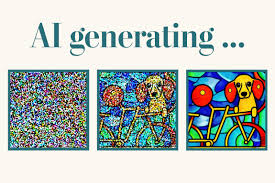
\includegraphics[height=4cm,width=6cm]{Picture/Ai.png}
\caption{图像去模糊化}
\end{minipage}%
\begin{minipage}[t]{0.45\linewidth}
\centering
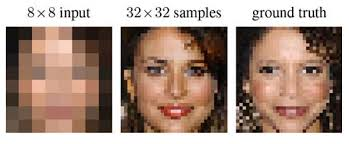
\includegraphics[height=4cm,width=6cm]{Graduation_thesis/Picture/imagerestore.png}
\caption{图像修复}
\end{minipage}
\end{figure}
在图像处理和分析的广泛领域中,图像质量无疑扮演着举足轻重的角色。对于后续的诸多处理任务,如特征提取、对象检测以及图像识别等,高质量的图像输入是确保任务准确性和鲁棒性的关键。有效实施图像去噪算法,能够显著减少图像中的噪声干扰,从而极大地改善这些后续处理任务的效果。去噪后的图像更加清晰、细节更丰富,使得算法能够更准确地捕捉到图像中的关键信息,提高特征匹配的精确度,增强对象检测的可靠性,以及优化图像识别的性能。因此,图像去噪不仅是提升图像质量的重要步骤,更是优化后续处理任务效果的必要手段。          

引领深度学习在图像处理领域的革新,无疑为图像处理技术的发展注入了新的活力。当我们将VAE(变分自编码器)和Diffusion Model等前沿的深度生成模型应用于图像去噪时,不仅能够克服传统去噪方法的局限性,还能大幅度提升去噪的效率和准确性。

首先,VAE作为一种强大的生成模型,其能够学习并捕捉图像数据的内在结构和特征。在图像去噪任务中,VAE可以通过对低质量图像进行编码和解码,去除其中的噪声,同时保留图像的原始信息。这使得去噪后的图像不仅清晰度高,而且细节丰富,为后续的图像处理任务提供了更好的基础。

而Diffusion Model则以其独特的扩散和去噪过程,在图像生成领域取得了显著的成果。将其应用于图像去噪,可以通过逐步去除图像中的噪声,逐渐还原出清晰的图像。这种渐进式的去噪方式,不仅能够有效去除各种复杂的噪声,还能保持图像的完整性和连贯性,使得去噪后的图像更加自然和真实。

通过将深度学习引入图像去噪领域,我们不仅能够提升去噪效果,还能进一步推动深度学习技术在图像处理领域的广泛应用。深度学习模型的强大学习和表征能力,使得我们能够更深入地挖掘图像数据的潜在信息,发现其中隐藏的规律和模式。这为我们开发更加智能化、高效化的图像处理算法提供了可能。

例如,在图像分割、目标检测等任务中,深度学习模型可以自动学习并识别图像中的关键特征和结构,从而实现更准确的分割和检测。在图像超分辨率、图像修复等任务中,深度学习模型则可以通过学习和重建图像的高频细节,使得图像更加清晰和真实。这些应用不仅提高了图像处理的效率和准确性,还为我们提供了更多的可能性和创新空间。

总之,结合VAE和Diffusion Model等深度生成模型进行图像去噪,不仅推动了深度学习在图像处理领域的应用,也为图像处理技术的发展带来了新的机遇和挑战。我们有理由相信,在未来的图像处理领域,深度学习将会发挥更加重要的作用,为我们带来更多的惊喜和成果。          



在众多实际应用的场景中,图像质量往往承载着至关重要的信息,特别是在医学影像、卫星图像分析以及安防监控等领域。在这些场景中,图像的清晰度和准确性直接关系到医疗诊断的精准性、地理信息的精确提取以及安全监控的有效性。因此,图像质量的保障对于决策和诊断来说,其重要性无法被忽视。

在医学影像领域,图像去噪算法的应用可以显著提高CT、MRI等医学影像的清晰度,帮助医生更准确地识别病变区域,从而做出更为精准的诊断。在卫星图像分析领域,图像去噪技术能够去除大气干扰、云层遮挡等噪声,使得卫星图像中的地理特征更加清晰,为城市规划、环境监测等提供有力支持。而在安防监控领域,图像去噪则能够提升监控视频的清晰度,有助于发现异常情况和安全隐患,保障公共安全。

为了满足这些实践应用的需求,开发高效准确的图像去噪算法显得尤为重要。这些算法需要能够针对不同应用场景的特点和需求,实现快速、有效的图像去噪处理。同时,随着深度学习等先进技术的不断发展,未来的图像去噪算法将更加智能化和高效化,为实际应用提供更加强大的支持。     


      综上所述,深入研究和探索图像去噪算法的重要性不言而喻。首先,这种研究能够显著提升图像的质量,无论是从视觉感受还是技术层面,都能使图像更为清晰、真实,进而极大地改善用户的观感和体验。其次,高质量的图像对于后续的图像处理任务至关重要,如特征提取、对象检测、图像识别等,都能因图像去噪而提高准确性和鲁棒性。

更重要的是,随着深度学习技术的迅猛发展,图像去噪算法的研究也为其在图像处理领域的应用开辟了新的道路。深度学习技术强大的学习和表征能力,使得我们能够更深入地挖掘图像数据的潜在信息,为图像去噪提供更加高效、智能的解决方案。这不仅推动了深度学习技术在图像处理领域的应用,同时也为图像处理领域带来了新的挑战和机遇。

最后,从实践应用的角度来看,图像去噪算法的研究也满足了众多领域对高质量图像的需求。在医学影像、卫星图像、安防监控等关键领域,图像质量直接关系到决策和诊断的准确性。因此,研究和开发高效准确的图像去噪算法,对于满足实际应用的需求,具有重要的理论价值和实践意义。

综上所述,图像去噪算法的研究不仅关乎图像质量的提升和后续处理任务的效果,更是推动深度学习技术在图像处理领域应用的关键,同时也满足了实际应用的需求,具有深远的理论和实践意义。
\subsection*{本研究的目的}
本研究致力于深度探索VAE(变分自编码器)与Diffusion Model这两种前沿的深度生成模型如何协同工作,以优化图像去噪的处理流程。我们认识到,图像去噪不仅关乎技术层面的优化,更关系到图像真实性与细节的保持,这对于许多实际应用场景具有关键意义。

通过综合VAE的自编码器结构和Diffusion Model的概率建模能力,我们旨在实现一种新型的图像去噪框架。VAE以其强大的编码-解码能力,能够有效地捕捉图像的内部结构信息,而Diffusion Model则擅长于从噪声中逐步还原出清晰图像,其概率建模能力为我们提供了从噪声中恢复图像细节的可能。

我们期望这一结合能够实现对不同类型噪声的鲁棒去除,无论是常见的随机噪声还是复杂的结构噪声,都能通过我们的算法得到有效的抑制。同时,我们注重在去除噪声的过程中保持图像的真实性和细节,避免过度平滑或引入不必要的失真。

本研究不仅局限于图像去噪这一单一任务,其潜在影响可能延伸至图像增强、图像重建等更广泛的领域。我们希望通过这一研究,为这些领域提供新的视角和方法,推动相关技术的发展。

更重要的是,通过对图像去噪问题的深入研究,我们期待为实际应用场景提供更加鲁棒和可靠的解决方案。无论是在医学影像、卫星遥感还是安防监控等领域,高质量的图像都是做出准确决策和诊断的基础。因此,我们的研究成果有望推动计算机视觉技术在实践中的广泛应用和进一步发展。
\section{研究现状与难点}
当下使用深度学习模型来处理图像生成尽管已经获得了巨大的成功,依然有一些最基本的问题仍然没有得到充分的解决。        


\textbf{表达能力}:在当前的研究领域中,如何运用深度学习模型来灵活适应不同图像生成问题的具体场景,已成为一项至关重要的议题。尽管神经网络的理论基础表明,一个深度和宽度足够大的神经网络能够以任意精度逼近任意函数,但这同时也意味着训练任务的复杂性和计算资源的消耗将显著增加。因此,在现有计算资源的限制下,如何更加高效地运用深度学习方法来有效解决具体问题,已成为当前研究的焦点之一。   


\textbf{图像生成算法}:面对当前热门的扩散模型如DDPM存在的采样时间过长问题——即使是在高质量图像生成时也需要近千步的采样过程,这无疑对计算资源和时间提出了巨大的挑战。如何在保持图像质量的同时,缩短生成时间、减少资源消耗,成为了对现有算法进行优化的关键。这不仅需要在算法层面上进行深入研究,还需要结合具体的下游任务需求,进行有针对性的改进和优化,以实现更高效、更实用的图像生成过程。 








\section{本文研究主要贡献}
本文的贡献主要集中在以下几个方面,显著推动了图像去噪和生成领域的研究与实践:

首先,针对深度学习模型在处理含噪声图像时的不鲁棒性,本文提出了一种新颖的基于扩散模型的图像去噪算法。这一算法的核心在于对后验分布似然函数的精确逼近,通过这种方法,算法能够稳定地去除图像中的噪声,还原出清晰的图像内容。与传统的去噪模型相比,本文提出的算法不仅具有更强的表达能力和更广泛的适用性,而且其函数族严格包含了已有模型的函数族,进一步提升了算法的灵活性和准确性。

其次,针对DDPM(去噪扩散概率模型)采样方法在训练过程中开销大的问题,本文创新性地采用了DDIM(去噪扩散隐式模型)中的采样方法,实现了分段采样策略。通过这一策略,算法能够显著减少迭代次数,降低在生成图片数量较大时的训练成本。这一改进不仅提高了图像修复算法的效率,也使得算法在实际应用中更具可行性。

最后,针对条件生成算法在采样速度和学习率调整方面的挑战,本文提出了一种无模型依赖的学习率设置算法。该算法通过动态调整学习率,以适应不同数据集和生成任务的需求。经过在LSUN、Imagenet及FFHQ等多个数据集上的实验验证,该算法显著提高了条件生成算法的稳定性,使得生成的图像质量更高、更符合实际需求。这一贡献对于推动条件生成算法的发展具有重要意义。
\section{论文结构安排}
首先,在第二章中,我们深入剖析了从传统的非条件生成模型,特别是变分自编码器(VAE),到当代先进的扩散模型在图像修复领域的演进脉络。我们详细回顾了VAE在图像处理领域的早期应用,评估了其在捕捉数据集复杂分布方面的强大能力,同时也指出了其存在的局限性。随着深度学习技术的蓬勃发展,扩散模型,尤其是Score-Based模型和Denoising Diffusion Probabilistic Models (DDPMs),在无监督学习框架下展现出卓越的数据分布学习能力,证明了其相较于传统模型的优越性。此外,本章还对最新的stable diffusion模型进行了重点评述,这一融合了扩散过程和深度学习技术的创新模型,在图像修复任务中展现出高效性和创新性,进一步推动了无监督学习算法在图像修复领域的应用和发展。

第三章则聚焦于本文的核心问题——图像修复的下游任务。我们首先从定义图像修复的具体场景和挑战入手,详细阐述了本文旨在解决的问题,即在给定前向加噪算子信息的情况下,如何通过加噪后的图像在目标数据集中生成满足后验关系的原像。接着,我们明确了本文的研究目标,即提高修复质量、缩短处理时间,并减少所需的计算资源,以满足实际应用中的高效和准确性需求。

第四章中,我们提出了本文的关键算法——基于条件生成的高效率图像修复算法。该算法通过精确估计后验概率分布,利用逆向SDE进行条件生成,从而实现图像修复的目的。为了验证算法的有效性,我们分别在FFHQ数据集和LSUN Bedrooms数据集上进行了测试,并展示了修复效果的对比图和与其他图像修复算法的效果对比。实验结果表明,我们的算法在图像修复任务中取得了显著的优势。

在第五章中,我们详细阐述了实验的设计和参数设置,介绍了在实现工程化图像去噪任务中所采用的技术和工具。通过严谨的实验设计和详尽的参数记录,我们确保了实验的可重复性和准确性。接着,我们对不同的条件生成模型进行了性能比较,采用了定量指标和定性分析相结合的方式,全面评估了所提出方法的优势。对比分析涵盖了生成图像的清晰度、色彩保真度、结构一致性等多个维度,进一步验证了我们的算法在图像修复任务中的优越性。

在最后的章节中,我们对图像修复领域的未来发展进行了展望和预测。我们讨论了潜在的技术突破方向,如通过深度学习进一步优化模型的结构、引入更先进的正则化技术,以及利用未来可能出现的计算资源等。这些技术突破有望进一步提升图像修复算法的性能和效率,推动图像修复领域的发展和应用。同时,我们也提出了一些建议,希望能为未来的研究和实践提供有益的参考。
% \section{引言的写法}

% 一篇学位论文的引言大致包含如下几个部分:
% 1、问题的提出;
% 2、选题背 景及意义;
% 3、文献综述;
% 4、研究方法;
% 5、论文结构安排。
% \begin{itemize}
%   \item 问题的提出:要清晰地阐述所要研究的问题“是什么”。
%     \footnote{选题时切记要有“问题意识”,不要选不是问题的问题来研究。}
%   \item 选题背景及意义:论述清楚为什么选择这个题目来研究,即阐述该研究对学科发展的贡献、对国计民生的理论与现实意义等。
%   \item 文献综述:对本研究主题范围内的文献进行详尽的综合述评,“述”的同时一定要有“评”,指出现有研究状态,仍存在哪些尚待解决的问题,讲出自己的研究有哪些探索性内容。
%   \item 研究方法:讲清论文所使用的学术研究方法。
%   \item 论文结构安排:介绍本论文的写作结构安排。
% \end{itemize}
